\documentclass[11pt]{article}
\usepackage[margin=1in]{geometry}
\usepackage[hidelinks]{hyperref}
\usepackage{amsmath}
\usepackage{graphicx}
\usepackage{tikz}
\usetikzlibrary{positioning,arrows.meta,fit}

\title{Keep the Recording or Write It Down?\\ A Matched-Budget Test of Audio Memory in Speech LLMs}
\author{Hanyu Yang}
\date{October 2026}

\begin{document}
\maketitle

\begin{abstract}
A speech assistant that remembers past conversations can keep the old audio or write it down. We compare
the two at equal cost in context positions on VoxMem 8K, and the answer depends on the reader. For
MiniCPM-o 4.5, write it down. Swapping part of a labelled text record for old clips, at the same total size,
changes accuracy by +0.7 points (95\% interval $-3.2$ to $+5.6$; 300 question families). Even a bare
transcript is no more than 10 points worse than the full audio history. For Gemini 3.8 Flash, in an
exploratory 48-family study, keep the audio for now. It scores 18.8 points higher with audio than with a
bare transcript. Text with speaker, emotion and sound labels matches the audio on average (43.8\% against
41.7\%), but the interval is too wide to call it a replacement. By our estimate the labelled text needs about 1/300 of the audio's storage, yet
its median memory takes about 45\% more context positions.
\end{abstract}

\section{Introduction}

Can a speech assistant forget your voice and still remember how you sounded? We test this on frozen speech
language models that answer questions about earlier sessions: who spoke, in what mood, over what background
sound.

The question matters because audio is expensive to keep. In MiniCPM-o a minute of speech fills about 600
context positions.

Xiao, Sethu and Holden built VoxMem to measure this kind of memory~\cite{voxmem}. They report that a
transcript alone fails on its acoustic questions: Gemini 3.7 Flash falls from 46.2\% with audio to 4.4\%
with text.

A transcript drops what the questions ask about. We tag every user turn with speaker, emotion and
sound-event labels from off-the-shelf models~\cite{sensevoice,emotion2vec,ast,wavlm} and store them as a few
lines of text. The fair comparison is then at equal cost: the same number of context positions spent on
text only, or partly on old clips.

We run it under two preregistrations, on 300 test families and 142 held-out families, with the open reader
MiniCPM-o 4.5. An exploratory study on 48 of the held-out families adds a closed reader, Gemini 3.8 Flash.
Our answer: for the open reader, old audio adds nothing measurable once the text carries labels. For the
strong reader, audio beats a transcript, and labelled text closes the gap on average but not yet with
confidence.

\section{What we did}

Each VoxMem item is a synthesized multi-session conversation at the 8K length, followed by a spoken question
about an earlier turn. We use the answerable acoustic questions and split them by question family. Filler
sessions recur across splits; evidence sessions do not.

A writer reads each session once, in order (Fig.~\ref{fig:pipeline}). For every user turn it stores its own
transcript and key--value labels; together these form the text record $M$. The budget is
$B_f = P_M + \lceil f P_A \rceil$, where $P_M$ is the size of $M$ in MiniCPM-o positions, $P_A$ the size of
the user audio, and $f = 0.25$. The memory arms are:
\begin{itemize}
\item $N$: no memory, only the question.
\item $M_{\mathrm{asr}}$: the transcript alone, without labels (holdout only).
\item $A$: the full audio history with the assistant's text turns, the VoxMem setting.
\item $T^*$: $M$ plus per-turn prosody numbers, filled to $B_f$.
\item $G$: the same text plus old user clips kept online by hash-priority eviction, filled to the same
  $B_f$ for each family. Audio is about 9\% of it (Fig.~\ref{fig:composition}).
\item $F$: $T^*$ plus every user clip, over budget.
\end{itemize}
Every memory is re-read from scratch for each question.

\begin{figure}[t]
\centering
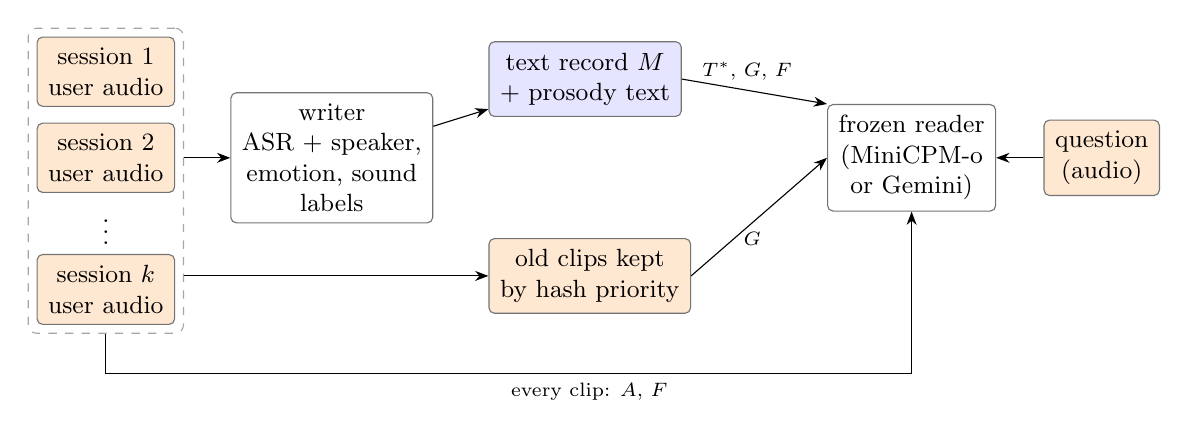
\begin{tikzpicture}[font=\small, >=Stealth, node distance=4mm and 7mm,
  box/.style={draw=black!55, rounded corners=2pt, align=center, inner sep=4pt, fill=white},
  aud/.style={box, fill=orange!18}, txt/.style={box, fill=blue!10}]
\node[aud] (s1) {session 1\\user audio};
\node[aud, below=2mm of s1] (s2) {session 2\\user audio};
\node[below=0mm of s2] (dots) {$\vdots$};
\node[aud, below=0mm of dots] (sk) {session $k$\\user audio};
\node[draw=black!35, dashed, rounded corners=3pt, fit=(s1)(sk), inner sep=3pt] (hist) {};
\node[box, right=of s2] (w) {writer\\ASR + speaker,\\emotion, sound\\labels};
\node[txt, right=of w, yshift=10mm] (m) {text record $M$\\+ prosody text};
\node[aud, right=of w, yshift=-15mm] (g) {old clips kept\\by hash priority};
\node[box, right=50mm of w] (r) {frozen reader\\(MiniCPM-o\\or Gemini)};
\node[aud, right=6mm of r] (q) {question\\(audio)};
\draw[->] (hist.east |- w.west) -- (w);
\draw[->] (hist.east |- g.west) -- (g.west);
\draw[->] (hist.south) -- ++(0,-5mm) -| node[pos=0.3, below, font=\scriptsize]{every clip: $A$, $F$} (r.south);
\draw[->] (w) -- (m);
\draw[->] (m.east) -- node[above, font=\scriptsize, pos=0.45]{$T^*$, $G$, $F$} (r.north west);
\draw[->] (g.east) -- node[below, font=\scriptsize, pos=0.45]{$G$} (r.west);
\draw[->] (q) -- (r);
\end{tikzpicture}
\caption{The memory pipeline. The writer passes once over the sessions. The reader gets the question after one of: the text record ($T^*$),
the text plus kept clips ($G$), the text plus every clip ($F$), or every clip with the assistant's text ($A$).}
\label{fig:pipeline}
\end{figure}

\begin{figure}[t]
\centering
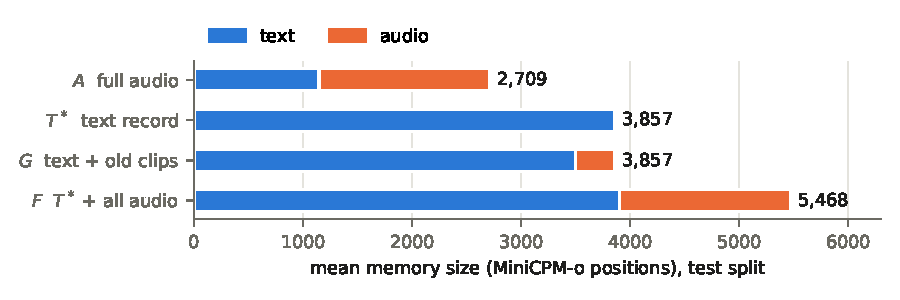
\includegraphics[width=\linewidth]{fig_composition.pdf}
\caption{Mean memory size per arm on the test split, divided into text and audio positions. $T^*$ and $G$ have the same size
for every family, to within one position. Text in $A$ is the assistant's turns; in $F$ it includes one
delimiter position per clip.}
\label{fig:composition}
\end{figure}

Settings were chosen on a 32-family dev split and frozen before the test split was run. The text side was
tuned over about nine settings and the audio policy over two.

The primary test was a gate: $F$ must significantly beat $T^*$ before we claim an audio benefit. If it does
not, $G - T^*$ is reported as an estimate only. On the holdout, the primary test asks whether
$M_{\mathrm{asr}}$ is at most 10 points worse than $A$, a one-sided non-inferiority test.

A first judge scores every answer blind to the arm: Gemini 3.8 Flash for MiniCPM-o's answers and Claude
Opus 5.5 for Gemini's, so that no model grades itself. A second judge sees a seeded 10\% plus every answer
where the first judge and a strict string matcher disagree. Intervals come from a type-stratified cluster
bootstrap. Clustering families by shared voice or background clip merged nearly everything, so the
preregistered fallback of one dominant source per family gave 48 units on test and 35 on holdout.

Gemini runs through an agent command-line tool that opens each clip as a file. It sees the same memories,
so its budgets are counted in MiniCPM-o positions.

\section{What we found}

\begin{figure}[!htb]
\centering
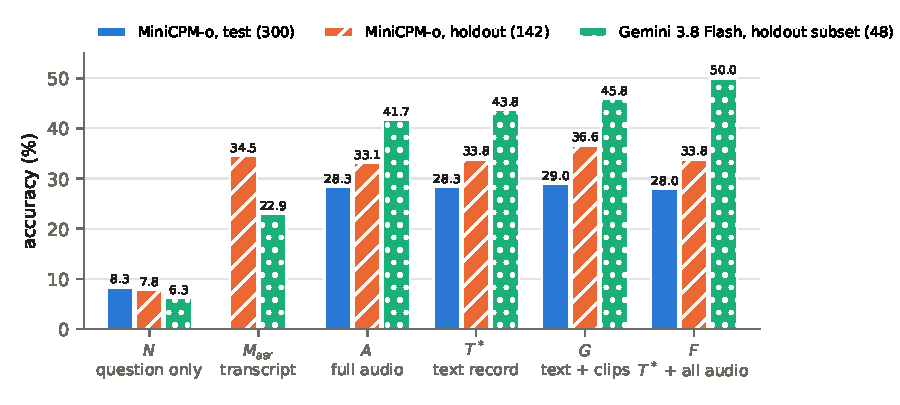
\includegraphics[width=\linewidth]{fig_accuracy.pdf}
\caption{Accuracy by memory arm under each reader's first judge. The Gemini bars cover 48 of the 142
holdout families. The test study has no transcript arm.}
\label{fig:accuracy}
\end{figure}

\begin{figure}[!htb]
\centering
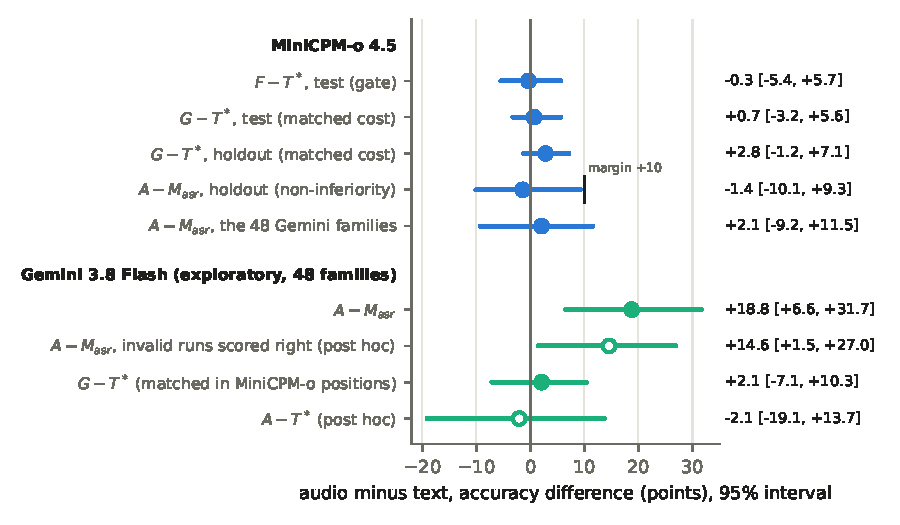
\includegraphics[width=\linewidth]{fig_contrasts.pdf}
\caption{Paired differences, each oriented as audio minus text, so points to the right favour audio.
Bars are 95\% type-stratified cluster-bootstrap intervals. On the non-inferiority row the tick marks the margin,
$A - M_{\mathrm{asr}} \le +10$; open circles are post hoc.}
\label{fig:contrasts}
\end{figure}

Figure~\ref{fig:accuracy} gives every accuracy and Figure~\ref{fig:contrasts} every comparison.

\textbf{MiniCPM-o: old audio adds nothing measurable.} $F - T^* = -0.3$ points ($-5.4$ to $+5.7$), so the gate
is not passed. At equal cost, $G - T^* = +0.7$ ($-3.2$ to $+5.6$) on test, which rules out a gain of 6
points there. On the holdout it is $+2.8$ ($-1.2$ to $+7.1$), and $+4.2$ ($0.4$ to $8.3$; sign-flip
$p = 0.053$) with the second judge's verdicts substituted where it saw the answer.

\textbf{MiniCPM-o: a bare transcript is non-inferior to full audio.} $A - M_{\mathrm{asr}} = -1.4$
($-10.1$ to $+9.3$). The upper bound clears the 10-point margin by 0.7 points. Separately, adding one label
group at a time to the transcript passed none of its tests.

\textbf{Gemini: audio beats a transcript.} Gemini scores 18.8 points higher with audio than with the
transcript ($6.6$ to $31.7$), against 2.1 for MiniCPM-o on the same families. The difference between the
readers is $+16.7$ ($5.6$ to $43.7$; $p = 0.032$), and $+14.6$ ($4.8$ to $31.3$) when both are scored by
the matcher. The agent could reach the answer file through shell commands, and every run that used them
answered exactly the gold. Two such runs remain, both transcript-only, and are scored wrong as
preregistered. Scored right, the audio gain is $+14.6$ ($1.5$ to $27.0$; $p = 0.057$).

\textbf{Gemini: labelled text matches audio on average, with wide uncertainty.} $T^*$ reaches 43.8\%
against 41.7\% for full audio, but $A - T^*$ spans $-19.1$ to $+13.7$. Old clips on top of the text add $+2.1$ ($-7.1$ to $+10.3$) at equal size in MiniCPM-o
positions.

\textbf{The text record is cheap to store, not to read.} By the repository's estimate (4 bytes per text
position, 16-bit audio), $T^*$ needs about 1/300 of the storage of the raw audio. In the reader it takes
about 45\% more positions than the full audio history.

The strict matcher disagrees with the first judge on 21--25\% of answers outside the question-only arm, and
puts MiniCPM-o's full-audio accuracy at 4.7\%. The gate, the non-inferiority result and the sign of Gemini's
audio gain are the same under all three scorings.

\section{Where this stops}

We did not test a retained key--value cache. The freeze record comes from a private repository and is
self-attested. On the holdout, the voice clustering behind the resampling units agreed with
itself within sessions only 89\% of the time, clip matching was 0.58, and the
non-inferiority margin is cleared by under a point. The Gemini result rests on one agent harness, 48
families, and budgets measured in another model's positions.

What we cannot say is why Gemini hears more in the audio. Our Gemini runs have no label ablations, so the
next study should ask which labels carry the cue and how few positions they need.

\paragraph{Data and code.}\sloppy\ \url{https://github.com/SeverinVisionary/voxmem-audio-vs-text-memory} holds
the code, both preregistrations, every reader answer and verdict, this paper with the script that draws its
figures, and a script that recomputes the reported statistics.

\begin{thebibliography}{9}
\bibitem{voxmem} Y.~Xiao, V.~Sethu, E.-J.~Holden et al. VoxMem: Benchmarking multimodal memory in large audio
language models. arXiv:2609.32607, 2026.
\bibitem{sensevoice} K.~An, Q.~Chen, C.~Deng et al. FunAudioLLM: Voice understanding and generation foundation
models for natural interaction between humans and LLMs. arXiv:2407.04051, 2024.
\bibitem{emotion2vec} Z.~Ma, Z.~Zheng, J.~Ye et al. emotion2vec: Self-supervised pre-training for speech
emotion representation. arXiv:2312.15185, 2023.
\bibitem{ast} Y.~Gong, Y.-A.~Chung, J.~Glass. AST: Audio spectrogram transformer. arXiv:2104.01778, 2021.
\bibitem{wavlm} S.~Chen, C.~Wang, Z.~Chen et al. WavLM: Large-scale self-supervised pre-training for full stack
speech processing. arXiv:2110.13900, 2021.
\end{thebibliography}

\end{document}
